\documentclass[UTF8,12pt]{article} % 12pt 为字号大小
\usepackage{amssymb,amsfonts,amsthm}
%\usepackage{fontspec,xltxtra,xunicode}
%\usepackage{times}
\usepackage{amsmath,bm}
\allowdisplaybreaks[4]
\usepackage{mdwlist}
\usepackage[colorlinks,linkcolor=blue]{hyperref}
\usepackage{cleveref}
\usepackage{enumerate}
\usepackage{extarrows}

%----------
% 定义中文环境
%----------

\usepackage{xeCJK}
\usepackage{float}
\setCJKmainfont[BoldFont={Heiti SC Light},ItalicFont={Kaiti SC Regular}]{Songti SC Regular}
\setCJKsansfont{Heiti SC Light}
\setCJKfamilyfont{song}{Songti SC Regular}
\setCJKfamilyfont{zhhei}{Heiti SC Light}
\setCJKfamilyfont{zhkai}{Kaiti SC Regular}
\setCJKfamilyfont{zhfs}{STFangsong}
\setCJKfamilyfont{zhli}{Libian SC Regular}
\setCJKfamilyfont{zhyou}{Yuanti SC Regular}

\newcommand*{\songti}{\CJKfamily{zhsong}} % 宋体
\newcommand*{\heiti}{\CJKfamily{zhhei}}   % 黑体
\newcommand*{\kaiti}{\CJKfamily{zhkai}}  % 楷体
\newcommand*{\fangsong}{\CJKfamily{zhfs}} % 仿宋
\newcommand*{\lishu}{\CJKfamily{zhli}}    % 隶书
\newcommand*{\yuanti}{\CJKfamily{zhyou}} % 圆体

%----------
% 版面设置
%----------
%首段缩进
\usepackage{indentfirst}
\setlength{\parindent}{2em}

%行距
\renewcommand{\baselinestretch}{1.5} % 1.5倍行距

%页边距
\usepackage[a4paper]{geometry}
\geometry{verbose,
  tmargin=2cm,% 上边距
  bmargin=2cm,% 下边距
  lmargin=2.5cm,% 左边距
  rmargin=2.5cm % 右边距
}


%----------
% 其他宏包
%----------
%图形相关
\usepackage[x11names]{xcolor} % must before tikz, x11names defines RoyalBlue3
\usepackage{graphicx}
\graphicspath{{figures/}}
\usepackage{pstricks,pst-plot,pst-eps}
\usepackage{subfig}
\def\pgfsysdriver{pgfsys-dvipdfmx.def} % put before tikz
\usepackage{tikz}

%原文照排
\usepackage{verbatim}

%网址
\usepackage{url}

%----------
% 定理、习题与解答环境
%----------
%定理环境
\usepackage[most]{tcolorbox}
\newtcbtheorem[number within=section]{theorem}{定理}{
     enhanced,
     breakable,
     sharp corners,
     attach boxed title to top left={
       yshifttext=-1mm
     },
     colback=blue!4!white,
     colframe=blue!75!black,
     fonttitle=\bfseries,
     boxed title style={
       sharp corners,
       size=small,
       colback=blue!75!black,
       colframe=blue!75!black,
     } 
}{theorem}

\newtcbtheorem[number within=section]{definition}{定义}{
     enhanced,
     breakable,
     sharp corners,
     attach boxed title to top left={
       yshifttext=-1mm
     },
     colback=blue!4!white,
     colframe=blue!75!black,
     fonttitle=\bfseries,
     boxed title style={
       sharp corners,
       size=small,
       colback=blue!75!black,
       colframe=blue!75!black,
     } 
}{definition}

\newtcbtheorem[number within=section]{corollary}{推论}{
     enhanced,
     breakable,
     sharp corners,
     attach boxed title to top left={
       yshifttext=-1mm
     },
     colback=blue!4!white,
     colframe=blue!75!black,
     fonttitle=\bfseries,
     boxed title style={
       sharp corners,
       size=small,
       colback=blue!75!black,
       colframe=blue!75!black,
     } 
}{corollary}

\newtcbtheorem[number within=section]{myboxes}{盒子}{
     enhanced,
     breakable,
     sharp corners,
     attach boxed title to top left={
       yshifttext=-1mm
     },
     %colback=white,
     colframe=black!75!white,
     fonttitle=\bfseries,
     boxed title style={
       sharp corners,
       size=small,
       colback=black!75!white,
       colframe=black!75!white,
     } 
}{myboxes}

%习题环境
\newtcbtheorem[]{exercise}{题}{
     enhanced,
     breakable,
     sharp corners,
     attach boxed title to top left={
       yshifttext=-1mm
     },
     colback=white,
     colframe=black,
     fonttitle=\bfseries,
     boxed title style={
       sharp corners,
       size=small,
       colback=black,
       colframe=black,
     } 
}{Problem}

%解答环境
\ifx\proof\undefined\
\newenvironment{proof}[1][\protect\proofname]{\par
\normalfont\topsep6\p@\@plus6\p@\relax
\trivlist
\itemindent\parindent
\item[\hskip\labelsep
\scshape
#1]\ignorespaces
}{%
\endtrivlist\@endpefalse
}
\fi

\renewcommand{\proofname}{\it{Solution}}

%----------
%示例:
%\begin{exs} \end{exs}
%\begin{proof}[] \end{proof}
%\begin{thm}{}{} \end{thm}
%----------

%----------
%插入图片
%\begin{figure}[htbp]
%\centering
%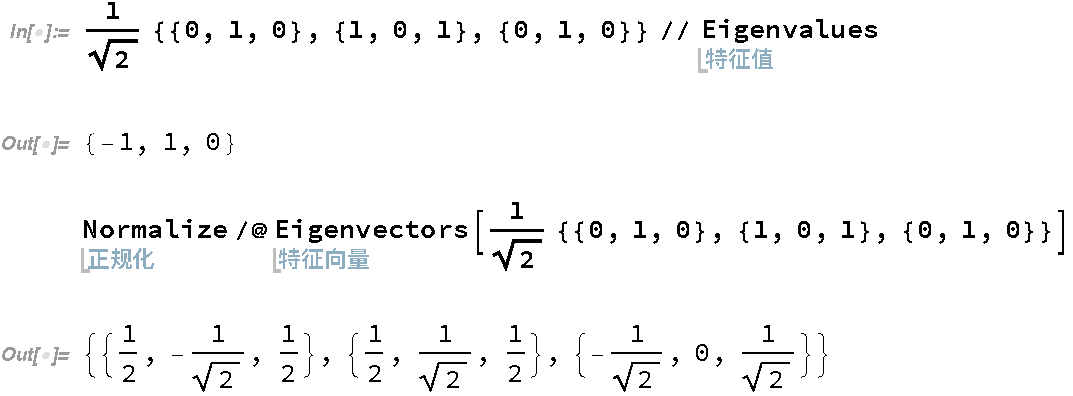
\includegraphics[width=10cm]{eigen}
%\end{figure}
%----------

%==========
% 正文部分
%==========

\begin{document}

\title{作业 08}
\author{陈昱全~SA18234049}
\date{} % 若不需要自动插入日期,则去掉前面的注释;{ } 中也可以自定义日期格式
\maketitle

\begin{exercise}{}{}
$A = \begin{pmatrix}1&1\\1&1\end{pmatrix}$, find eigenvalue $\lambda$, eigenstates $|\lambda\rangle$ of $A$. With $\sigma_{z} = \begin{pmatrix}1&0\\0&-1\end{pmatrix}$, show
$$\sigma_{z} \otimes A = \begin{pmatrix}1&1&0&0\\1&1&0&0\\0&0&-1&-1\\0&0&-1&-1\end{pmatrix},$$
find eigenvalue and eigenvectors of $\sigma_{z}\otimes A$, show the relation with $\pm\lambda$, and $|0\rangle|\lambda\rangle$, $|1\rangle|\lambda\rangle$.
\end{exercise}

\begin{proof}[解]
已知$A = \begin{pmatrix}1&1\\1&1\end{pmatrix}$,则本征值和本征态为
\begin{figure}[H]
\begin{center}
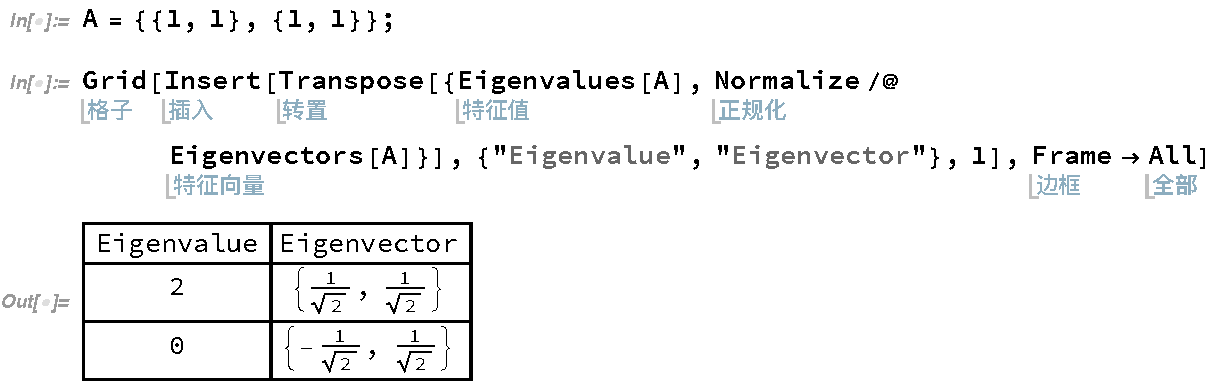
\includegraphics[width=14cm]{A}
%\caption{}
%\label{}
\end{center}
\end{figure}
又$\sigma_{z} = \begin{pmatrix}1&0\\0&-1\end{pmatrix}$,二者的直积$\sigma_{z} \otimes A$为
\begin{figure}[H]
\begin{center}
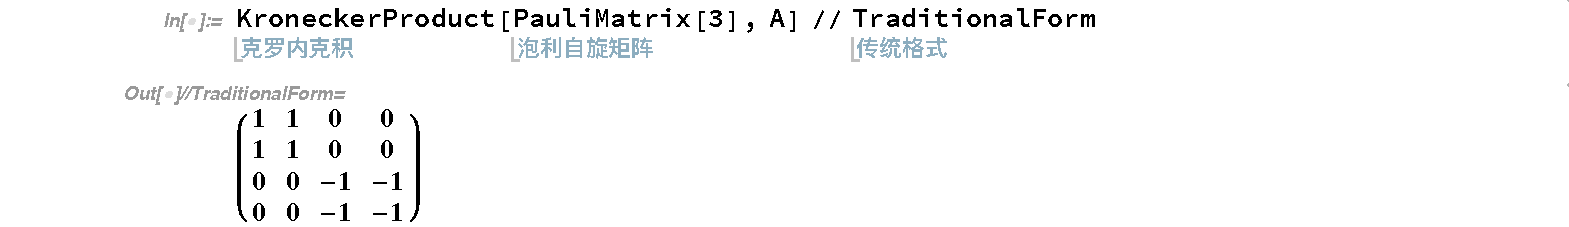
\includegraphics[width=17cm]{otimes}
%\caption{}
%\label{}
\end{center}
\end{figure}
同理,可以求得$\sigma_{z} \otimes A$的本征值和本征态,
\begin{figure}[H]
\begin{center}
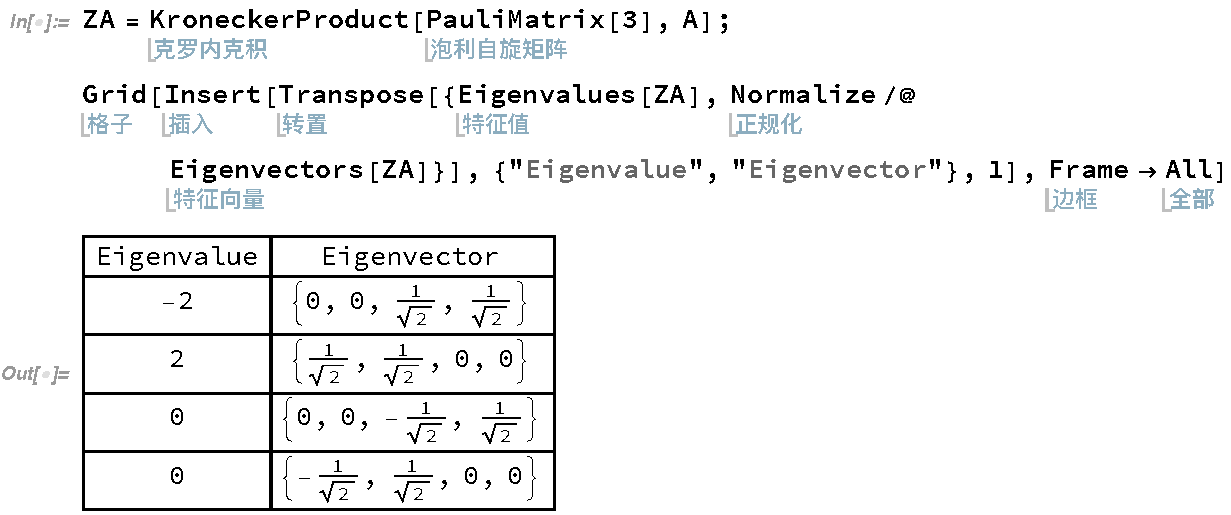
\includegraphics[width=14cm]{ZA}
%\caption{}
%\label{}
\end{center}
\end{figure}
易知,$\sigma_{z} \otimes A$的本征值和本征态有如下关系:
\begin{table}[H]
%\caption{default}
\begin{center}
\begin{tabular}{|c|c|}\hline
本征值 & 本征态\\\hline
$\lambda$ & $|0\rangle|\lambda\rangle$\\\hline
$-\lambda$ & $|1\rangle|\lambda\rangle$\\\hline
\end{tabular}
\end{center}
%\label{default}
\end{table}

\end{proof}


\begin{exercise}{}{}
``w-state'', for N-spin-$\frac{1}{2}$ particles, one can construct
$$|w_{N}\rangle \equiv \frac{1}{\sqrt{N}}(|10...0\rangle + |010...0\rangle + ... + |0...01\rangle)$$
with all the permutation of one of the particles at state $|1\rangle$ and the other particles at $|0\rangle$ state. What is the probability of measuring $|1\rangle$ state for the first particle? If we measure $|0\rangle$ for the first particle, find the relation of the remaining state and $|w_{N-1}\rangle$.
\end{exercise}

\begin{proof}[解]
由于$|w_{N}\rangle = \frac{1}{\sqrt{N}}(|10...0\rangle + |010...0\rangle + ... + |0...01\rangle)$,对$|w_{N}\rangle$进行测量,有$\frac{1}{N}$的概率得到态$|10...0\rangle$,即测量到第一个粒子状态为$|1\rangle$的概率为
\begin{align}
P_{\text{第一个粒子为}|1\rangle} = \frac{1}{N}
\end{align}
如果测量第一个粒子得到状态$|0\rangle$,则测量之后体系的状态变为
\begin{align}
|w_{N}'\rangle &= \sqrt{\frac{N}{N-1}} \frac{1}{\sqrt{N}}(|010...0\rangle + |0010...0\rangle + ... + |0...01\rangle) \\
&= \frac{1}{\sqrt{N-1}}(|010...0\rangle + |0010...0\rangle + ... + |0...01\rangle) \\
&= |0\rangle \otimes \frac{1}{\sqrt{N-1}}(|10...0\rangle + |010...0\rangle + ... + |0...01\rangle) \\
&= |0\rangle \otimes |w_{N-1}\rangle
\end{align}
\end{proof}


\begin{exercise}{}{}
Evolution of coupled spin-$\frac{1}{2}$ system.
$$H = \Omega(\sigma_{z}\otimes I + I\otimes \sigma_{z}),~ |\psi(t=0)\rangle = \frac{1}{\sqrt{2}}(|01\rangle + |10\rangle),$$
find $|\psi(t)\rangle$.\\
Hint: find the eigenstates and eigenvalues of $H$ first
\end{exercise}

\begin{proof}[解]
可以先求出哈密顿量$H$的本征值和本征态,然后利用
\begin{align}
e^{\hat{A}} = \sum_{i} e^{A_{i}}|i\rangle\langle i|
\end{align}
来求得时间演化算符$U(t) = e^{-\frac{i}{\hbar}Ht}$。用Mathematica来求解的话,可以直接求得$U(t)$:
\begin{figure}[H]
\begin{center}
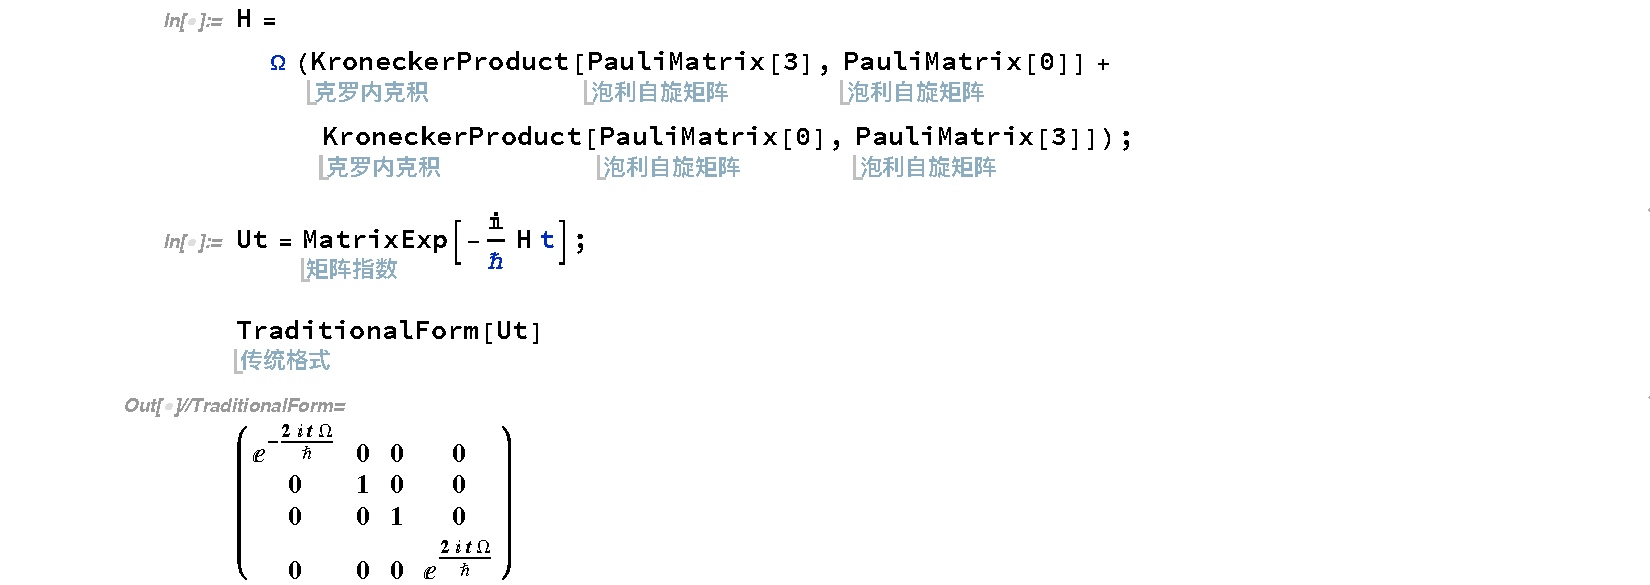
\includegraphics[width=19cm]{ut}
%\caption{}
%\label{}
\end{center}
\end{figure}
代入$|\psi(0)\rangle = \frac{1}{\sqrt{2}}(|01\rangle + |10\rangle)$,可得$|\psi(t)\rangle$为:
\begin{figure}[H]
\begin{center}
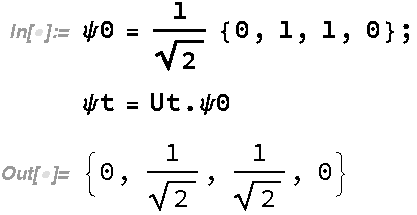
\includegraphics[width=4.5cm]{psit}
%\caption{}
%\label{}
\end{center}
\end{figure}
\end{proof}



\end{document}